% 1.Introduction
% ====================================================================
\section{Introduction}
\label{sec:introduction}
        
In this work, we present a bound on the criticality of \demorgan formulas. We build on a key lemma from \hastad's work on the shrinkage exponent of \demorgan formulas~\cite{hastad1998shrinkage}, which bounds the probability of a formula reducing to a literal under random restrictions. This lemma serves as the base case for our main theorem. We extend the concept of a formula simplifying to a literal by adapting the notion of Canonical Decision Trees (CDT) for Formulae from previous works by ~\cite{rossmanCriticalityRegularFormulas2019}, ~\cite{harshaCriticalityAC0Formulae2023}. 
% ====================================================================
We also introduce a structural result for Boolean formulas under random restrictions, which we call the Banyan decomposition ~\cref{lem:banyan}. This decomposition allows us to reduce the event of a CDT of a formula having a long path to several sub-formulae having reducing to a literal under appropriate restrictions. Furthermore, the notion of downward closure from previous works ~\cite{hastad2014parity}, ~\cite{harshaCriticalityAC0Formulae2023} allows us to treat these events on the sub-formulae as if they  were independent events. 
The main proof delicately puts together of all these ideas and  makes them work together.

\begin{theorem}
\label{thm: main}
    Let $\Lfunc \in \mathbb{N}$, $p \in (0,1)$, $t \in \N$. Let $F$ be a \demorgan formula with $\Lfunc$ leaves and $\calR_p$ be the $p$-random restriction.
    $$\Pr_{\rho \in \calR_p}[\DTdepth(F|_\rho) \geq t] \leq (p\sqrt{\Lfunc})^t$$
\end{theorem}

% --- 1.1 Organization ---
\subsection{Organization}
\label{sec:organization}
This paper is organized as follows:
\begin{itemize}
    \item \Cref{sec:preliminaries} provides the necessary preliminary definitions and concepts, including \demorgan formulae, random restrictions, and decision tree depth, downward closure, trunk and aerial roots. 
    \item \Cref{sec:cdt} introduces our Canonical Decision Tree ($\CDT$) construction, along with the subroutines $\zeroBal$ and $\oneBal$. 
    \item \Cref{sec:unpacking} contains the Unpacking lemma and the Banyan decomposition. 
    \item \Cref{sec:proof-main-theorem} presents the detailed proof of our main theorem, outlining the structural lemma, properties of twin-leaved trees, and the probabilistic calculations using convexity arguments.
    \item  \Cref{sec: Hastad's base case proof} contains the base case proof \hastad. 
\end{itemize}

% \begin{table}[h!]
% \centering
% \begin{tabular}{|l|l|}
% \hline
% \textbf{Notation} & \textbf{Description} \\
% \hline
% \multicolumn{2}{|l|}{\textbf{Basic Concepts}} \\
% \hline
% $F$ & A de Morgan formula. \\
% $\rho$ & A restriction on the variables of $F$. \\
% $X$ & The set of variables of a formula. \\
% $F|_{\rho}$ & The formula $F$ with restriction $\rho$ applied. \\
% \hline
% \multicolumn{2}{|l|}{\textbf{Decision Trees and Paths}} \\
% \hline
% $\CDT(F, \rho)$ & The Canonical Decision Tree for $F$ under restriction $\rho$. \\
% $\alpha = (x_1 \gets a_1, \dots, x_t \gets a_t)$ & An ordered restriction, representing a path of length $t$. \\
% $\alpha[s, t]$ & The sub-path of $\alpha$ from index $s$ to $t$. \\
% $\CDT_z^{(a)}(F, \rho) = \alpha$ & The event that $\CDT(F, \rho)$ takes a path $\alpha$ to a leaf with value $z$. \\
% \hline
% \multicolumn{2}{|l|}{\textbf{Balancing Subroutines and Association}} \\
% \hline
% $\zeroBal(\Gamma)$ & The subroutine to \zeroBal a decision tree $\Gamma$. \\
% $\oneBal(\Gamma)$ & The subroutine to 1-balance a decision tree $\Gamma$. \\
% $\Assoc(\Gamma, \alpha)$ & The function returned by the balance subroutines; maps a path $\alpha$ \\
% & to its unique associated path in the balanced tree $\Gamma$. \\
% $Assoc_{\to 1}(F, \rho, \alpha)$ & The high-level notation for $\Assoc(\zeroBal(\CDT(F, \rho)), \alpha)$. \\
% $\Assoc_1(F, \rho, \alpha)$ & The high-level notation for $\Assoc(\oneBal(\CDT(F, \rho)), \alpha)$. \\
% \hline
% \multicolumn{2}{|l|}{\textbf{Banyan Decomposition}} \\
% \hline
% $T$ & The trunk of the Banyan decomposition, a subtree of the formula tree. \\
% $t(v)$ & The number of aerial roots under a node $v$ in the trunk. \\
% $\alpha(v)$ & The pre-restriction on the subformula at a node $v$. \\
% $\beta(v)$ & The original path assignment for the variables under $v$. \\
% $vars(v)$ & The sequence of variables picked by the CDT algorithm from under $v$. \\
% \hline
% \end{tabular}
% \end{table}





% ====================================================================
% Preliminaries
% ====================================================================
\section{Preliminaries}
\label{sec:preliminaries}

For a positive integer $n \in \N$, $[n]$ refers to the set $\set{1, 2, \dots, n}$. All logarithms in this paper are to
base 2.

We use bold letters to represent a random sample drawn from a distribution, differentiating it from a fixed element of the sample space. For any distribution $D$ on a finite set $\Sigma$, we denote its probability mass function by $\mu_D$. Here, $\mu_D(\sigma)$ gives the probability of drawing the specific element $\sigma$ from the distribution $D$. We'll drop the subscript from $\mu$ when the distribution is clear from the context. 

In this section, we define key objects and concepts used throughout the paper. We begin by recalling the definition of a \demorgan formula.

\begin{definition}[\demorgan Formula]  %---\demorgan Formula ---%
\label{def:demorgan_fomula}
A \emph{\demorgan formula} is a boolean formula composed of $\lor$ (OR), $\land$ (AND), and $\neg$ (NOT) gates. NOT gates are only allowed on the leaf variables (literals). All internal gates have fan-in 2, which implies that the formula can be represented as a binary tree whose leaves are labeled by literals (variables or their negations).
\begin{enumerate}
    \item The \textbf{size} of a \demorgan formula $F$ is denoted by $\Lfunc(F)$, which is the number of leaves in its binary tree representation. 
    \item The \textbf{depth} of a \demorgan formula is the length of the longest path from the root to any leaf in its binary tree representation.
    \item For a subformula $G$ of $F$ and a variable $x$, we denote by $\Lfunc(G, x)$ the number of leaves in $G$ that are labeled by the variable $x$ (either as $x$ or $\neg x$). We will typically drop the subformula $G$ from the notation and write $\Lfunc(x)$ when $G$ is the main formula $F$ and the context is clear.
\end{enumerate}
\end{definition}

\begin{definition}[Restriction] %---Restriction ---%
\label{def:restriction}
Given a variable index set $X$, a \emph{restriction} $\rho$ is a function $\rho: X \to \{0, 1, \star\}$ or, equivalently, a partial function from $X$ to $\{0, 1\}$. We refer to the domain of this partial function as $\operatorname{dom}(\rho)$ and the remaining set of unrestricted variables, namely $X \setminus \operatorname{dom}(\rho)$, as $\operatorname{stars}(\rho)$.
\begin{itemize}
    \item We say that two restrictions $\rho_1$ and $\rho_2$ are \emph{consistent} if for every $v \in \operatorname{dom}(\rho_1) \cap \operatorname{dom}(\rho_2)$, we have $\rho_1(v) = \rho_2(v)$.
    \item We can define a partial ordering among restrictions as follows: we say $\rho_1 \preceq \rho_2$ if (1) $\operatorname{dom}(\rho_2) \subseteq \operatorname{dom}(\rho_1)$ and (2) $\rho_1$ and $\rho_2$ are consistent. In words, $\rho_1$ "sets more variables" than $\rho_2$. Sometimes, we will only be interested in this order with respect to a particular subset $T$ of the variable index set $X$. In this case, we say $\rho_1 \preceq_T \rho_2$ if (1) $\operatorname{dom}(\rho_2) \cap T \subseteq \operatorname{dom}(\rho_1) \cap T$ and (2) $\rho_1$ and $\rho_2$ are consistent.
\end{itemize}

Given a formula $F$ and a restriction $\rho$, the \emph{restricted formula} $F|_{\rho}$ refers to the formula obtained by relabeling literals involving variables in $\operatorname{dom}(\rho)$ according to $\rho$ (we make no further simplification to the formula). Given two consistent restrictions $\rho_1, \rho_2$, $F|_{\rho_1, \rho_2}$ refers to the formula $(F|_{\rho_1})|_{\rho_2}$ (which is identical to $(F|_{\rho_2})|_{\rho_1}$).
\end{definition}

\begin{definition}[Random Restriction]  %---p Random Restriction ---%
\label{def:random-restriction}
A \emph{$p$-random restriction}, denoted by $\calR_p$, is a distribution over restrictions where each variable $x_i \in X$ is independently assigned a value according to the following probabilities:
\begin{itemize}
    \item $x_i$ is set to $\star$ (unassigned) with probability $p$.
    \item $x_i$ is set to $0$ with probability $(1-p)/2$.
    \item $x_i$ is set to $1$ with probability $(1-p)/2$.
\end{itemize}
\end{definition}

\begin{definition}[Ordered Restriction]  %--- Ordered Restriction ---%
\label{def:ordered-restriction}
An \emph{ordered restriction} on a variable set $X$ is a sequence of the form $\alpha = \abra{x_{1} \to b_1, \dots, x_{t} \to b_t}$ where $t \in \mathbb{N}$, $b_i \in \{0, 1\}$, and $x_1, \dots, x_t$ are distinct elements of $X$. We will use $\operatorname{dom}(\alpha)$ to refer to the set $\{x_{1}, \dots, x_{t}\}$. (We will typically use $\alpha$ or $\beta$ for ordered restrictions.)

We sometimes ignore the order of variables in an ordered restriction $\alpha$ and use the same variable name $\alpha$ to denote the unordered restriction.
% Similarly, given a restriction $\rho$ on $X$, and an ordering on $\operatorname{dom}(\rho)$, we have a natural representation of $\rho$ as an ordered restriction on $X$.
\end{definition}

\begin{definition}[Decision Tree]
\label{def:decision-tree}
A \emph{decision tree} is a finite rooted binary tree where
\begin{itemize}
    \item each internal node is labeled by a variable from a set $X$ and has exactly two children, with the edges to its children labeled $0$ and $1$, respectively. The variables appearing in any root-to-leaf path are distinct.
    \item the leaves are labeled by a constant value from $\{0, 1\}$.
\end{itemize}
The depth of a decision tree $T$, denoted by $\DTdepth(T)$, is the maximum number of internal nodes along any root-to-leaf path in $T$.

A decision tree $T$ is said to compute a Boolean function $f \colon \{0,1\}^n \to \{0,1\}$ if for every assignment $\sigma \in \{0,1\}^n$, the path from the root of $T$ corresponding to the assignments in $\sigma$ terminates at a leaf labeled $f(\sigma)$.
\end{definition}

\begin{definition}[Criticality]
\label{def:criticality}
The criticality of a Boolean function $f$, as defined by Rossman \cite{rossmanCriticalityRegularFormulas2019}, is the smallest real number $\lambda$ such that for every $p \in (0,1)$ and every integer $t \geq 0$, we have
\[
\Pr_{\rho \sim \calR_p}[\DTdepth(f|_{\rho}) \geq t] \leq (p\lambda)^t
\]
\end{definition}
We are interested in studying the criticality of \demorgan formulae. It has been conjectured by Rossman in ~\cite{rossmanCriticalityRegularFormulas2019}  that the Criticality of \demorgan formula of size $\Lfunc$ is $O(\sqrt{\Lfunc})$. We address this question in the positive in this paper. 

\begin{definition}[Downward-Closed Set of Restrictions]
\label{def:downward-closed}
Let $\Delta$ be a set of restrictions on a variable set $X$, and let $T \subseteq X$ be a subset of the variables. We say that the set $\Delta$ is \emph{downward-closed with respect to $T$} if for any pair of restrictions $\rho, \rho' \in \Delta$, the following holds:
$$
\rho \in \Delta \text{ and } \rho' \preceq_T \rho \implies \rho' \in \Delta
$$
Informally, if a restriction is in the set, then any restriction that sets more variables from $T$ while remaining consistent is also in the set. When the context is clear, we will simply refer to the set as being downward-closed.
\end{definition}

% % \begin{definition}[Trunk and Dangling Sub-formulae]
% % \label{def:trunk-and-dangling}
% % Given a formula $F$, we will abuse notation and refer to its underlying tree structure also as $F$. A \emph{Trunk} is a sub-tree of $F$ that has the same root as $F$ and whose terminal nodes are internal nodes of the original tree $F$. The sub-trees of $F$ rooted at these terminal nodes are called \emph{Dangling sub-trees}.
% % \end{definition}

\begin{definition}[Trunk, Dangling Sub-trees, and Aerial Roots]
\label{def:trunk-and-dangling}
Given a formula $F$, we will abuse notation and refer to its underlying tree structure also as $F$. A \emph{Trunk} $\T$ is a sub-tree of $F$ that has the same root as $F$ and whose terminal nodes are internal nodes of the original formula $F$ with the property that the sibling of each terminal node in $\T$ also belongs to the trunk $\T$. 
The sub-trees of $F$ rooted at these terminal nodes are called \emph{Dangling sub-trees}, and their roots are referred to as \emph{aerial roots}.
\end{definition}

\paragraph{Notation}
We understand that the notation we use is new to the reader, so we provide a table which keeps track of all the notation.
\begin{table}[h!]
\centering
\begin{tabular}{|l|l|}
\hline
\textbf{Notation} & \textbf{Description} \\
\hline
\multicolumn{2}{|l|}{\textbf{Basic Concepts}} \\
\hline
$F$ & A \demorgan formula. \\
$X$ & The set of variables of a formula. \\
$\Lfunc(F)$ & The size of a formula $F$, defined as the number of leaves. \\
$\Lfunc(x)$ & Number of leaves labeled $x$ (or $\neg x$). \\
$\Lfunc(G, x)$ & The number of leaves in subformula $G$ labeled by variable $x$. \\
\hline
\multicolumn{2}{|l|}{\textbf{Restrictions}} \\
\hline
$\rho$ & A restriction on the variables of $F$. \\
$F|_{\rho}$ & The formula $F$ with restriction $\rho$ applied. \\
$\operatorname{dom}(\rho)$ & The set of variables fixed by $\rho$. \\
$\operatorname{stars}(\rho)$ & The set of variables left unassigned ($\star$) by $\rho$. \\
$\rho \sim \mathcal{R}_p$ & A $p$-random restriction, where each variable is independently $\star$ with probability $p$. \\
$\Delta$ & A downward-closed set of restrictions. \\
\hline
\multicolumn{2}{|l|}{\textbf{Decision Trees and Paths}} \\
\hline
$\CDT(F, \rho)$ & The Canonical Decision Tree for $F$ under restriction $\rho$. \\
$\alpha = (x_1 \gets a_1, \dots, x_t \gets a_t)$ & An ordered restriction, representing a path of length $t$. \\
$\alpha[s, t]$ & The sub-path of $\alpha$ from index $s$ to $t$. \\
$\DTdepth(T)$ & The depth of a decision tree $T$. \\
$\CDT_z^{(a)}(F, \rho) = \alpha$ & The event that $\CDT(F, \rho)$ takes a path $\alpha$ to a leaf with value $z$. \\
$\Pi_F$ & The Karchmer-Wigderson protocol for $F$. \\
\hline
\multicolumn{2}{|l|}{\textbf{Balancing Subroutines and Association}} \\
\hline
$\zeroBal(\Gamma)$ & The subroutine to $\zeroBal$ a decision tree $\Gamma$. \\
$\oneBal(\Gamma)$ & The subroutine to 1-balance a decision tree $\Gamma$. \\
$\Assoc(\Gamma, \alpha)$ & A function that maps a path $\alpha$ to its unique associated path in the balanced tree $\Gamma$. \\
$Assoc_{\to 1}(F, \rho, \alpha)$ & High-level notation for $\Assoc(\zeroBal(\CDT(F, \rho)), \alpha)$. \\
$\Assoc_1(F, \rho, \alpha)$ & High-level notation for $\Assoc(\oneBal(\CDT(F, \rho)), \alpha)$. \\
\hline
\multicolumn{2}{|l|}{\textbf{Banyan Decomposition and Certificates}} \\
\hline
$\T$ & The trunk of the Banyan decomposition, a subtree of the formula tree. \\
$t(v)$ & The number of aerial roots under a node $v$ in the trunk. \\
$\alpha(v)$ & The pre-restriction on the subformula at a node $v$. \\
$\beta(v)$ & The original path assignment for the variables under $v$. \\
$\mathrm{vars}(v)$ & The sequence of variables picked by the CDT algorithm from under $v$. \\
$\EC(\T, \bT, \bar{x})$ & An exploration certificate for a Trunk $\T$. \\
$\mathcal{A}_F$ & A condition related to the $\Assoc$ procedure in the Banyan Decomposition. \\
$\mathcal{B}_F$ & A condition related to literal simplification at aerial roots in the Banyan Decomposition. \\
\hline
\multicolumn{2}{|l|}{\textbf{Probabilistic Analysis}} \\
\hline
$E_{\Delta}(x, \ell)$ & An event relating a random restriction to a specific leaf $\ell$ and variable $x$. \\
\hline
\end{tabular}
\end{table}


% ====================================================================
% Canonical Decision Tree
% ====================================================================
\section{Canonical Decision Tree (CDT)}
\label{sec:cdt}


A central component of our proof is the construction of a appropriate canonical decision tree for a \demorgan formula $F$ under a restriction $\rho$.
This is inspired by constructions of Canonical Decision Trees for various other classes of functions such as $\CNF$s,$\DNF$s from the works of ~\cite{hastad1986smalldepththesis} ~\cite{razborov1993equivalence} ~\cite{beame1994switching}  and $\AC^0$ formulae from the works of~\cite{rossmanCriticalityRegularFormulas2019}, ~\cite{hastad2014parity}. Our choice of CDT for \demorgan formula can be seen as a special case of the $\AC^0$ Formula $\CDT$ used by ~\cite{rossmanCriticalityRegularFormulas2019} and ~\cite{harshaCriticalityAC0Formulae2023}. We use a single restriction for the whole as opposed a chain or a tree of restriction to construct our $\CDT$.

% --- CDT for DNFs and CNFs ---
\subsection{CDT for depth 2 formulae}
A main idea in the all these constructions of all these CDTs is the notion of balancing. Let us see the CDT construction and Balancing in the case of DNFs and use that to motivate the Balancing and CDT construction for \demorgan formulae. 

\begin{algorithm}[H]
    \caption{$\CDT(F, \rho)$: Canonical Decision Tree for DNF}
    \label{alg:dnf-cdt}
    \textbf{Input:} A DNF $F = T_1 \lor \dots \lor T_m$, and a restriction $\rho$. \\
    \textbf{Output:} A decision tree for $F|_{\rho}$.
    \begin{algorithmic}[1]
        \Statex \textbf{Step 1.} Select Term and Handle Base Cases
        \State Find the first term $T$ (from left to right) that is not forced to $0$ by $\rho$.
        \If {no such term exists}
            \State \Return a single leaf node labeled $0$. \mycomment{in this case, $F|_\rho \equiv 0$}
        \EndIf
        \If {$T|_{\rho} \equiv 1$}
            \State \Return a single leaf node labeled $1$. \mycomment{in this case, $F|_\rho \equiv 1$}
        \EndIf
        
        \Statex \textbf{Step 2.} Construct CDT of the Term
        \State Let $Y$ be the set of variables in $T$ that are unrestricted by $\rho$.
        \State Construct a decision tree $\Gamma$ from the complete balanced binary tree on the variables of $Y$.
        
        \Statex \textbf{Step 3.} Recurse
        \For {each leaf $v$ of $\Gamma$}
            \State Let $\alpha_v$ be the ordered restriction corresponding to the path to $v$.
            \State Replace the leaf $v$ with a new decision tree: $\CDT(F|_{\alpha_v}, \rho)$.
        \EndFor
        \State \Return $\Gamma$.
    \end{algorithmic}
\end{algorithm}

Note that, in the above algorithm, instead of using the optimal algorithm for $T_i$, we non-adaptively query all the surviving variables of $T_i$ and for a complete binary tree. The reason we do this is to ensure, that every 1-path has a corresponding 0-path in the decision tree of $T_i$. This property turn out to be crucial in the proofs of all the existing Switching lemmas. We ensure that the  decision that we construct have this property by doing the balancing operations $\oneBal$ and $\zeroBal$.    


%%%% FOR A SINGLE "AND" TERM
\begin{figure}
    \centering
    \begin{subfigure}[h]{0.4\textwidth}
        \centering
        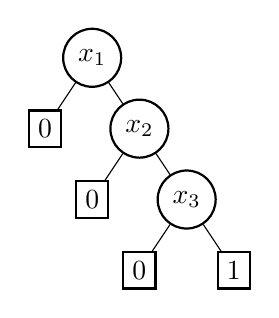
\begin{tikzpicture}[scale = 0.3, treenode/.style={circle, draw, thick}, leaf/.style={rectangle, draw, thick}]
        
        \node[treenode] at (2, 9) (x1){$x_1$};
        \node[leaf] at (0, 6) (leaf1) {0};
        \node[treenode] at (4, 6) (x2){$x_2$};
        \node[leaf] at (2, 3) (leaf2){0};
        \node[treenode] at (6, 3) (x3){$x_3$};
        \node[leaf] at (4, 0) (leaf3){0};
        \node[leaf] at (8, 0) (leaf4){1};
        
        \draw (x1) -- (leaf1);
        \draw (x1) -- (x2);
        \draw (x2) -- (leaf2);
        \draw (x2) -- (x3);
        \draw (x3) -- (leaf3);
        \draw (x3) -- (leaf4);   
        \end{tikzpicture}
        \caption{Optimal $\DT$ for $x_1\wedge x_2 \wedge x_3$}
    \end{subfigure}
    \hfill
    \begin{subfigure}[h]{0.4\textwidth}
        \centering
        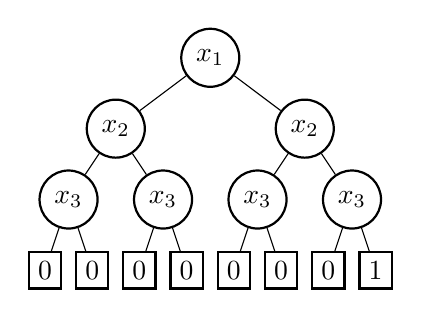
\begin{tikzpicture}[scale = 0.3, treenode/.style={circle, draw, thick}, leaf/.style={rectangle, draw, thick}]
        
        \node[treenode] at (9, 9) (x1){$x_1$};

        \node[treenode] at (5, 6) (x21) {$x_2$};
        \node[treenode] at (13, 6) (x22){$x_2$};

        \node[treenode] at (3, 3) (x31){$x_3$};
        \node[treenode] at (7, 3) (x32){$x_3$};
        \node[treenode] at (11, 3) (x33){$x_3$};
        \node[treenode] at (15, 3) (x34){$x_3$};

        \node[leaf] at (2, 0) (leaf1){0};
        \node[leaf] at (4, 0) (leaf2){0};
        \node[leaf] at (6, 0) (leaf3){0};
        \node[leaf] at (8, 0) (leaf4){0};
        \node[leaf] at (10, 0) (leaf5){0};
        \node[leaf] at (12, 0) (leaf6){0};
        \node[leaf] at (14, 0) (leaf7){0};     
        \node[leaf] at (16, 0) (leaf8){1};
        
        \draw (x1) -- (x21);
        \draw (x1) -- (x22);

        \draw (x21) -- (x31);
        \draw (x21) -- (x32);
        \draw (x22) -- (x33);
        \draw (x22) -- (x34);
        
        \draw (x31) -- (leaf1);
        \draw (x31) -- (leaf2);
        \draw (x32) -- (leaf3);
        \draw (x32) -- (leaf4); 
        \draw (x33) -- (leaf5);
        \draw (x33) -- (leaf6); 
        \draw (x34) -- (leaf7);
        \draw (x34) -- (leaf8);      
        \end{tikzpicture}
        \caption{Completed balanced $\DT$ for $x_1 \wedge x_2 \wedge x_3$}
    \end{subfigure}
    \caption{Illustration of $\DT(x_1\wedge x_2\wedge x_3)$ used in the $\CDT$ construction in the proof of \hastad's Switching Lemma.}
    \label{fig: term CDT}
\end{figure}


\subsection{Balancing}
% --- Balancing sub-section ---
Our $\CDT$ construction uses a balancing procedure to ensure certain structural properties.

\begin{algorithm}[H]
    \caption{$\zeroBal(\Gamma)$: Zero-Balancing Procedure}
    \label{alg:0-balancing}
    \textbf{Input:} A decision tree $\Gamma$. \\
    \textbf{Output:} A $\zeroBal$ d decision tree $\Gamma''$.
    \begin{algorithmic}[1]
        \Statex \textbf{Phase 1: Pruning and Initializing}
        \State Prune $\Gamma$ by replacing any subtree with all 0-leaves with a single 0-leaf to get $\Gamma'$.
        \Statex \textbf{Phase 2: Bottom-up Balancing}
        \State Let $d$ be the depth of $\Gamma'$ and let $\Gamma_{d} = \Gamma'$.
        \For {$i=d-1$ down to $1$}
        \Statex Stage $i$:
            \State Let $\Gamma_{i+1}$ be the intermediate tree obtained after stage $i+1$.
            \State Consider all $0$-leaves $u$ at distance $i$ from the root in $\Gamma_{i+1}$.
            \State Let $v$ be the sibling of $u$, and let $T_v$ be the subtree rooted at $v$.
            \State \mycomment{By construction, $T_v$ must contain at least one $1$-leaf.}
            \State Create a new subtree $T_v'$ by mirroring $T_v$ and relabeling all its leaves with $0$.
            \State Replace the leaf $u$ with the new subtree $T_v'$ in $\Gamma_{i+1}$ to get $\Gamma_i$.
        \EndFor
        \State \Return $\Gamma_1$.
    \end{algorithmic}
\end{algorithm}

\subsection{Finding the original path}

The \textbf{$\zeroBal$} procedure outputs a decision tree $\Gamma''$ such that every \textbf{0-path} in it is uniquely associated with a \textbf{1-path} that queries the exact same sequence of variables.

We now define a procedure called $\Assoc(F,\rho,\alpha)$ which, when given an ordered restriction $\alpha$ corresponding to a 0-path in $\Gamma'' = \zeroBal(\CDT(F,\rho))$, outputs the unique 1-path from which it was cloned.

This is accomplished with a subroutine called \textbf{findSource}, which takes a 0-path as input and returns the immediate source path from which it was cloned. The $\Assoc$ procedure is then defined by a repeated application of \textbf{findSource} until the unique 1-path is discovered.

\begin{claim}[Source of a Cloned Path]
\label{claim:cloned-path-source}
Let $\Gamma'' = \zeroBal(\CDT(F, \rho))$ be a $\zeroBal$ decision tree, and let $\alpha = (x_1 \gets a_1, \dots, x_t \gets a_t)$ be a path that terminates in a 0-leaf. Then there exists a unique index $i \in \{1, \dots, t\}$ such that the following two conditions hold:
\begin{enumerate}
    \item The path $\alpha' = (x_1 \gets a_1, \dots, x_i \gets 1 - a_i, \dots, x_t \gets a_t)$ is a valid path in $\Gamma''$ that terminates in a 1-leaf.
    \item For any index $j > i$, the path $\alpha_j' = (x_1 \gets a_1, \dots, x_j \gets 1 - a_j, \dots, x_t \gets a_t)$ is not a valid path in $\Gamma''$.
\end{enumerate}
\end{claim}

Let $\Gamma'' = \zeroBal(\CDT(F, \rho))$ be a $\zeroBal$ decision tree, and let $\alpha = (x_1 \gets a_1, \dots, x_t \gets a_t)$ be a path that terminates in a 0-leaf. Then there exists a unique highest-indexed variable $x_i$ such that the path prefix $(x_1 \gets a_1, \dots, x_i \gets a_i)$ corresponds to a leaf in the tree before stage $i$ of the balancing procedure, and at this node, the sub-formula evaluates to 0, while its sibling branch has a path to a 1-leaf.
The following subroutine finds this highest-indexed variable $x_i$ and there by find the immediate source path that it is cloned from. 

\begin{claim}[Source of a Cloned Path]
\label{claim:cloned-path-source-stage}
Let $F$ be a \demorgan formula, $\rho$ a restriction, and $\alpha = (x_1 \gets a_1, \dots, x_t \gets a_t)$ an ordered restriction such that $F|_{\rho \cup \alpha} \equiv 0$. Then there exists a unique highest-indexed variable $x_i$ and a restriction $\gamma = (v_{i+1} \gets c_{i+1}, \dots, x_t \gets c_t)$ such that the following two conditions hold:
\begin{enumerate}
    \item The prefix of the path $\alpha_i = (x_1 \gets a_1, \dots, x_i \gets a_i)$ is such that $F|_{\rho \cup \alpha_i} \equiv 0$.
    \item The path $\alpha_i' = (x_1 \gets a_1, \dots, x_i \gets 1 - a_i)$ extend with $\gamma$ leads to a 1-path, i.e. $F|_{\rho \cup \alpha_i' \cup \gamma}$ evaluates to $1$.
\end{enumerate}
\end{claim}

\begin{algorithm}[H]
    \caption{$\mathbf{findSource}(F, \rho, \alpha)$}
    \label{alg:find-source}
    \textbf{Input:} A \demorgan formula $F$, a restriction $\rho$, and a path $\alpha = (x_1 \gets a_1, \dots, x_t \gets a_t)$ corresponding to a 0-path.
    \textbf{Output:} The immediate source path $\alpha'$ from which $\alpha$ was cloned.
    \begin{algorithmic}[1]
        \For {$i=t$ down to $1$}
            \State Let $\alpha_i \gets (x_1 \gets a_1, \dots, x_i \gets a_i)$.
            \State Let $F_i \gets F|_{\rho \cup \alpha_i}$.
            \If {$F_i \equiv 0$}
                \State Let $\alpha'_i \gets (x_1 \gets a_1, \dots, x_i \gets 1 - a_i)$.
                \State Let $F'_i \gets F|_{\rho \cup \alpha'_i}$.
                \For {each assignment $\gamma$ to variables $(v_{i+1}, \dots, x_t)$}
                    \If {$F'_i|_{\gamma}$ evaluates to 1}
                        \State \Return $(x_1 \gets a_1, \dots, x_i \gets 1 - a_i, \dots, x_t \gets a_t)$.
                    \EndIf
                \EndFor
            \EndIf
        \EndFor
        \State \Return $\perp$ \Comment{Should not be reached for a valid 0-path.}
    \end{algorithmic}
\end{algorithm}

\begin{algorithm}[H]
    \caption{$Assoc_{\to 1}(F, \rho, \alpha)$: Finding the Associated 1-Path}
    \label{alg:assoc}
    \textbf{Input:} A \demorgan formula $F$, a restriction $\rho$, and a path $\alpha$ that terminates at a 0-leaf. \\
    \textbf{Output:} The unique 1-path $\beta$ associated with $\alpha$.
    \begin{algorithmic}[1]
        \State Let $\alpha_{current} \gets \alpha$.
        \While {the path $\alpha_{current}$ terminates at a 0-leaf}
            \State $\alpha_{current} \gets \findSource(F, \rho, \alpha_{current})$.
        \EndWhile
        \State \Return $\alpha_{current}$.
    \end{algorithmic}
\end{algorithm}

The $Assoc_{\to 1}$ procedure's behavior is well-defined for "honest" 0-paths, but it also behaves predictably for other types of paths.

\paragraph{Behavior on a 1-Path}
If the input $\alpha$ is an honest 1-path from the balanced decision tree $\Gamma''$, the \texttt{while} loop in the $Assoc_{\to 1}$ procedure will not execute even once. The loop's condition, "while the path $\alpha_{\text{current}}$ terminates at a 0-leaf," is immediately false.

In this case, the procedure simply returns the input path itself. This is the desired behavior for a 1-path, as it's already a source path and doesn't need any further processing.

\paragraph{Behavior on a Non-Existent Path}
If the input $\alpha$ is not a path at all in the balanced tree (e.g., a path that was pruned away or simply doesn't exist), the \texttt{findSource} subroutine's checks for formula equivalence will not work as intended. The logic assumes that for any 0-path, a corresponding 1-path exists.

The \texttt{findSource} routine will iterate through all possible variables. If it fails to find a valid pivot that leads to a 1-path, its \texttt{for} loop will complete, and the procedure will return $\perp$ (bottom), signaling that a source could not be found. This is the "bot" case, and it correctly indicates an error in the input.



\begin{algorithm}[H]
    \caption{$\CDT(F, \rho)$: Canonical Decision Tree for \demorgan Formulae}
    \label{alg:cdt-demorgan}
    \textbf{Input:} A \demorgan formula $F$, and a restriction $\rho$. \\
    \textbf{Output:} A decision tree for $F|_{\rho}$.
    \begin{algorithmic}[1]
        \Statex \textbf{Base Cases}
            \If {$F|_\rho$ is a constant}
                \State \Return a single leaf node with that constant value ($0$ or $1$).
            \EndIf
            \If {$F$ is a single literal ($x_i$ or $\neg x_i$)}
                \State \Return a decision tree for $x_i$, with leaves labeled $0$ and $1$.
            \EndIf
            
        \Statex \textbf{Recursive Step}
            \State Let $F = F_1 \lor F_2$ be the top-level gate.
            \If {$F_1|_\rho \equiv 0$}
                \State \Return $\CDT(F_2, \rho)$.
            \ElsIf {$F_1|_\rho \equiv 1$}
                \State \Return a single leaf node labeled $1$.
            \Else \quad \mycomment{Interesting case: $F_1|_\rho$ is non-constant}
                \State Let $\Gamma \gets \CDT(F_1, \rho)$. \mycomment{construct $\CDT$ of $F_1$}
                \State $\Gamma' \gets \zeroBal(\Gamma)$ \mycomment{Balancing step}
                \For {each $0$-leaf $v$ in $\Gamma'$}
                    \State Let $\alpha_v$ be the ordered restriction to $v$.
                    \State Replace leaf $v$ with the tree $\zeroBal(\CDT(F_2|_{\alpha_v}, \rho))$. \mycomment{attach $\zeroBal$ version of $\CDT$ of $F_2$} 
                \EndFor
                \State \Return $\Gamma'$.
            \EndIf
            
        \Statex \textbf{Symmetry for AND-gates}
        \State The case for $F = F_1 \land F_2$ is handled symmetrically by swapping the roles of $0$ and $1$ and using the $\oneBal$ balancing operation.
    \end{algorithmic}
\end{algorithm}
Whether we $\zeroBal$ or $\oneBal$ and the CDT of a formula $G$ is decided at the time of construction of the CDT of its parent. If the parent of $G$ is $\lor$, we $\zeroBal$ $\CDT(G,\rho)$ and if the parent of $G$ is $\land$, we $\oneBal$.  


\begin{definition}
    Let $F$ be a \demorgan formula and $\rho$ be a restriction, let $t$ be a non-negetive integer.  For any bit string $a \in \{0, 1\}^t$, let $\alpha_a$ be the ordered restriction obtained by traversing the path in the decision tree $\CDT(F, \rho)$ according to the sequence of bits in $a$.
    \begin{equation}
        \label{eq: CDTa}
        \CDT^{(a)}_z(F, \rho) =
        \begin{cases}
            \alpha_a & \text{if } F|_{\rho,\alpha_a} \equiv z \\
            \bot & \text{otherwise}
        \end{cases}
    \end{equation}
    If $t=0$, $a$ is the empty string and $\alpha$ is the empty ordered restriction, the condition $\CDT^{(a)}_z(F,\rho) = \alpha$ is defined to mean $F|_{\alpha,\rho} \equiv z$. 
\end{definition}

% ====================================================================
% Unpacking
% ====================================================================
\section{Unpacking}
\label{sec:unpacking}


\begin{lemma}[Unpacking for OR]
\label{lem:unpacking for OR}
    Let $F = F_1 \lor F_2$ be a \demorgan formula, $\rho$ be a restriction, $t \in \N$ and $a \in \zo^t$, $z \in \zo$. Let $\alpha$ be an ordered restriction of length $t$ given by $\alpha = \abra{x_1 \gets a_1, \dots, x_t \gets a_t}$ for some variables $x_1, \dots x_t \in X$.
    If $\CDT^{(a)}_z(F, \rho) = \alpha$ then one of the following mutually exclusive conditions holds:
    \begin{itemize}
        \item Case 1: $F_1|\rho \equiv 0$,
        $\bra{F_2|_{\alpha}}_\rho \equiv z$,  
        $\exists b \in \zo^t$ and $\beta = \abra{x_1 \gets b_1, \dots , x_t \gets b_t}$ such that $\CDT^{(b)}_1(F_2,\rho) = \beta$ and $Assoc_{\to 1}(F_2,\rho,\alpha) = \beta$. 
        % $\CDT^{(a)}_z(F_2,\rho) = \alpha$.
        \item Case 2: $\bra{F_1|_\alpha}|_{\rho} = 0$, $\exists b \in \zo^t$ and $\beta = \abra{x_1 \gets b_1, \dots , x_t \gets b_t}$ such that $\CDT^{(b)}_1(F_1,\rho) = \beta$ and $Assoc_{\to 1}(F_1, \rho , \alpha) = \beta$ and $(F_2|_\alpha)|_{\rho} \equiv z$. 
        \item Case 3: $\exists 0< s < t$, $b_1 \in \zo^s$ and $b_2 \in \zo^{t-s}$ such that by letting $\alpha_1 = \abra{x_1 \gets a_1, \dots x_s \gets a_s}$, $\alpha_2 = \abra{x_{s+1} \gets a_{s+1}, \dots x_t \gets a_t}$, $\beta_1= \abra{x_1 \gets b_1, \dots x_s \gets b_s }$ and $\beta_2 = \abra{x_{s+1} \gets b_{s+1}, \dots x_t \gets b_t}$ we have
        \begin{itemize}
            \item $\CDT^{(b_1)}_1(F_1,\rho) = \beta_1$ and $Assoc_{\to 1}(F_1,\rho,\alpha_1)=\beta_1$,
            \item $\CDT^{(b_2)}_1(F_2|_{\alpha_1},\rho) = \beta_2$ and $Assoc_{\to 1}(F_2|_{\alpha_1},\rho,\alpha_2)=\beta_2$
        \end{itemize}
    \end{itemize}
\end{lemma}
The case when $F  = F_1 \land F_2$ is similar with the roles of 0 and 1 interchanged.

\subsection{Banyan Decomposition}
Repeated application of the \cref{lem:unpacking for OR} give rise to a structural lemma, which we call as Banyan Decomposition. Given a trunk $\T$ and an assignment for each node $v$ in the trunk, we can define the following auxiliary  data which certifies the fact that $\T$ is the trunk uniques trunk associated with the long path $\alpha$ in $\CDT{F,\rho}$.

\begin{definition}[Exploration Certificate]
\label{def:draft-certificate}
Given a sequence of $t$ variables $\bar{x} = (x_1, \dots , x_t)$, a Trunk $\T$ and a collection of bit-strings $\bT = \{b_v\}_{v \in \T}$ for each node $v \in \T$, we define the \emph{Exploration Certificate} denoted by $\EC(\T, \bT,\bar{x})$ as the tuple $(t_v, X_v, \eta_v, \alpha_v, \beta_v)$ , where all its components which are defined below are functions of $\bar{x}$, $\T$, and $\bT$:
\begin{enumerate}
    \item \textbf{Length $t_v$:} $t_v(\T)$ is the number of terminal nodes of $\T$ under a node $v$.
    \item \textbf{Sub-sequence of Variables $X_v$:} Assign the variables of the sequence $\bar{x}$ to the terminal nodes of $\T$ based on the in-order on the nodes of $\T$. 
    $X_v(\T, \bar{x})$ is the sub-sequence of variables from $\bar{x}$ that are assigned to the terminal nodes of $\T$ under $v$.
    \item \textbf{Pre-restriction $\eta_v$:} A restriction defined recursively as follows, 
    if $v$ is the root of $\T$, $\eta_v = \abra{}$ and for all other nodes of $\T$,
    $\eta_v = \eta_{\parent(v)} \circ \alpha_{\lsibling(v)}$ if $v$ has a $\lsibling(v) \in \T$, else $\eta_v = \eta_{\parent(v)}$.  
    % \tm{alpha of the parent truncated} \todo
    \item \textbf{Original Path $\beta_v$:} A path defined as $\beta_v = \abra{X_v \gets b_v}$.
    \item \textbf{Inherited Path $\alpha_v$:} A path defined recursively as $\alpha_v = \beta_{\parent(v)}[1,t(v)]$, $\alpha(v) = \beta(v)$ if $v$ is the root. 
\end{enumerate}
The \emph{Exploration certificate} is the tuple $\EC(\T, \bT) = (t_v, X_v, \eta_v, \alpha_v, \beta_v)$.
\end{definition}

\begin{lemma}[Banyan Decomposition lemma]
\label{lem:banyan}
    Let $F$ be a \demorgan formula, and $\rho$ be a restriction. Let $t \in \N$,  let $\alpha = \abra{x_1 \gets a_1, \dots, x_t \gets a_t}$ for any bit string $a \in \zo^t$ and let $z \in \zo$.%be a path in $\CDT(F, \rho)$ for some variables $x_1, \dots, x_t$. 
    If $\CDT^{(a)}_z(F, \rho) = \alpha$, then there exist a unique Trunk $\T$ whose aerial roots $(v_1, \dots, v_t)$ correspond to variables $(x_1, \dots, x_t)$and a unique collection of bit-strings $\bT = \{b_v\}_{v \in \T}$ for each non-root, non-terminal node $v \in \T$ such that their corresponding exploration certificate $\EC(\T, \bT) = (t_v, X_v, \eta_v, \alpha_v, \beta_v)$, satisfies the following two conditions:
    \begin{itemize}
        \item $\calA_F(\rho,\bar{x}, \T, \bT)$: For each non-terminal node $v \in \T$, 
        \begin{itemize}
            \item if $F_v = F_{v_1} \lor F_{v_2}$, for $j \in \{1,2\}$, if $F_{v_j}|_{\rho,\eta_{v_j}} \equiv 0$ then $v_j \notin \T$, else if $F_{v_j}|_{\rho,\eta_{v_j}} \not\equiv 0$, it is witnessed by $F_{v_j}|_{\rho,\eta(v_j),\beta(v_j)} \equiv 1$ and $Assoc_{\to 1}(F_{v_j}|_{\eta_{v_j}}, \rho, \alpha_{v_j}) = \beta_{v_j}$.     
            \item if $F_v = F_{v_1} \land F_{v_2}$, for $j \in \{1,2\}$, if $F_{v_j}|_{\rho,\eta_{v_j}} \equiv 1$ then $v_j \notin \T$, else if $F_{v_j}|_{\rho,\eta_{v_j}} \not\equiv 1$, it is witnessed by $F_{v_j}|_{\rho,\eta(v_j),\beta(v_j)} \equiv 0$ and 
            $\Assoc_1(F_{v_j}|_{\eta_{v_j}}, \rho, \alpha_{v_j}) = \beta_{v_j}$.
        \end{itemize}
        \item $\calB_F(\rho,\bar{x}, \T, \bT)$: For each aerial root $v$ of the trunk $\T$, $CDT^{(a)}(F_v|_{\eta_v}, \rho) = (X_v \to a)$ for $a \in \zo$. 
        % the sub-formula $F_v$ simplifies to a literal under the given restriction: $ F_v|_{\rho \circ \eta_v} \text{ is a literal}$ in the single variable $X_v$.
    \end{itemize}
\end{lemma}

 
\begin{proof}[Proof of Banyan Decomposition]
The proof proceeds by induction on $t$ and the size of the formula. 
\paragraph{Base case:}
When $t=1$,\footnote{Note that this case also covers the other base case \ie when $F$ is a single node.} $F|_{\rho} \equiv x$ or $\neg x$ for some variable $x$. In this case $\T$ is the single node which the root of $F$, since there no non-terminals of $\T$, $\bT$ is the empty set.    

\paragraph{Induction hypothesis:} $\forall s\in [t]$, $\forall$ sub-formulae $G$ of $F$,\footnote{by sub-formulae, we not only mean the formulae corresponding to the sub-trees of $F$, but also their restricted versions with arbitrary pre-restrictions} if $\CDT^{(a)}_z(F,\rho) = (\bar{x} \gets a)$, 
there exists $\T_G$ and $\mathsf{b}_{\T_G}= \cbra{b}_{v \in \T_G}$  such that $\calA_G(\rho,\bar{x}, T_G, \mathsf{b}_{\T_G})$
and $\calB_G(\rho,\bar{x}, T_G, \mathsf{b}_{\T_G})$ are satisfied.

\paragraph{Induction step:} 
Suppose there exist $a \in \zo^t$ and variables $\bar{x}= (x_1, \dots ,x_t)$ such that $\CDT^{(a)}_z(F,\rho) = (\bar{x} \gets a)$. 
If $F = F_1 \vee F_2$, by \cref{lem:unpacking for OR}, there are three cases bases on the number of variables $s$ picked from $F_1$ in $\CDT(F,\rho)$.

\begin{itemize}
    \item \textbf{Case 1} (s= 0) $F_1|\rho \equiv 0$ and $\CDT^{(a)}_z(F_2,\rho) = \alpha$ and $\exists b \in \zo^t$, $\CDT^{(b)}_1(F_2,\rho) = \beta$ and $Assoc_{\to 1}(F_2, \rho , \alpha) = \beta$ and $(F_2|_\alpha)|_{\rho} \equiv z$
    In this case, by induction hypothesis there exists a trunk $\T_{F_2}$ and $\mathsf{b}_{\T_{F_2}}$ which satisfy the conditions $\calA_{F_2}$ and $\calB_{F_2}$. 
    $\T_F$ is the tree obtained by adding the root of $F$ to $T_{F_2}$. $\sfb_{F_2}(root(F_2)) = b$ and for all other internal of $T_F$,  $\sfb_{\T_F} = \sfb_{\T_{F_2}}$. 

    \item \textbf{Case 2:} (s=t)
   then $\exists b \in \zo^t$ and $\beta = \abra{x_1 \gets b_1, \dots , x_t \gets b_t}$ such that $\CDT^{(b)}_1(F_1,\rho) = \beta$ and $Assoc_{\to 1}(F_1, \rho , \alpha) = \beta$ and $(F_2|_\alpha)|_{\rho} \equiv z$. 
    By induction hypothesis there exists a trunk $\T_{F_1}$ and $\mathsf{b}_{\T_{F_1}}$ which satisfy the conditions $\calA_{F_1}$ and $\calB_{F_1}$. 
    $\T_F$ is the tree obtained by adding the root of $F$ to $T_{F_1}$. $\sfb_F(root(F_1)) = b$ obtained from the \cref{lem:unpacking for OR} and for all other internal of $T_F$, $\sfb_F = \sfb_{F_1}$.

    \item \textbf{Case 3:} then $\exists 0< s < t$, $b_1 \in \zo^s$ and $b_2 \in \zo^{t-s}$ such that by letting $\alpha_1 = \abra{x_1 \gets a_1, \dots x_s \gets a_s}$, $\alpha_2 = \abra{x_{s+1} \gets a_{s+1}, \dots x_t \gets a_t}$, $\beta_1= \abra{x_1 \gets b_1, \dots x_s \gets b_s }$ and $\beta_2 = \abra{x_{s+1} \gets b_{s+1}, \dots x_t \gets b_t}$ we have
    \begin{itemize}
        \item $\CDT^{(b_1)}_1(F_1,\rho) = \beta_1$ and $Assoc_{\to 1}(F_1,\rho,\alpha_1)=\beta_1$,
        \item $\CDT^{(b_2)}_1(F_2|_{\alpha_1},\rho) = \beta_2$ and $Assoc_{\to 1}(F_2|_{\alpha_1},\rho,\alpha_2)=\beta_2$                
    \end{itemize}
    Since $\CDT_1^{(b_1)}(F_1,\rho) = \beta_1$ and $\CDT_1^{(b_2)}(F_2|_{\alpha_1}) = \beta_2$, there exist $\T_{F_1}$, $\sfb_{T_{F_1}}$ which satisfy $\calA_{F_1}$, $\calB_{F_1}$ and  $\T_{F_2|_{\alpha_1}}$, $\sfb_{T_{F_2|_{\alpha_1}}}$ which satisfy $\calA_{F_2|_{\alpha_1}}$, $\calB_{F_2|_{\alpha_1}}$. We define $T$ with a new node as root and $\T_{F_1}$ and $\T_{F_2}$ as its left and right children respectively.  
    $\sfb_{\T}(v_{F_1}) = b_1$ and $\sfb_{\T}(v_{F_2}) = b_2$ where $v_{F_1}$ and $v_{F_2}$ are the roots of $F_1$ and $F_2$ respectively. 
    $\bT(v) = \sfb_{\T_{F_1}}(v)$ if $v \in F_1$ and $\bT(v) = \sfb_{\T_{F_1}}(v)$ if $v \in F_1$.
\end{itemize}

\end{proof}

% ====================================================================
% Main Proof
% ====================================================================
\section{Proof of the Main Theorem}
\label{sec:proof-main-theorem}

In order to bound the probability that the Decision tree depth of \demorgan formula $F$ under a $p$-random restriction is larger than $t$, it is enough to show this statement paths of length exactly $t$ and consider CDTs instead of the optimal decision trees. 



\begin{theorem}
\label{thm: intermediate}
    Let $\Lfunc,t \in \N$, $p \in (0,1)$, $a \in \zo^t$, $z \in \zo$. Let $F$ be a \demorgan formula with $\Lfunc$ leaves then   
    $$\Pr_{\rho \sim \calR_p}[\exists \alpha \CDT_z^{(a)}(F,\rho) = \alpha] \le (p \sqrt{\Lfunc})^t$$
\end{theorem}

\begin{proof}[Proof of Theorem \ref{thm: main}]

If the depth of the optimal decision tree for $F|_\rho$ is at least $t$, then so will be the depth of $\CDT(F,\rho)$.
Therefore

\begin{align}
    \Pr_{\rho \in \calR_p}[\DTdepth(F|_\rho) \ge t] &= \Pr_{\rho \in \calR_p}[\CDTdepth(F,\rho) \ge t] \\
    &\le \sum_{u \ge t} \Pr_{\rho \in \calR_p}[\CDTdepth(F,\rho) = u]\\
    % \intertext{This step uses the law of total probability, breaking down the total probability into a sum over all possible exact depths $u \ge t$.}
    &\le \sum_{u \ge t} \sum_z \sum_{a \in \zo^u} \Pr_{\rho}[\exists \alpha\CDT_z^{(a)}(F,\rho) = \alpha]
    \intertext{This step uses the union bound. The probability of the CDT having depth $u$ is bounded by the sum of probabilities of all possible paths of that length. The notation $\exists \alpha\CDT_z^{(a)}(F,\rho) = \alpha$ refers to the event that a path corresponding to the bit string $a$ exists and fixes the formula to the value $z$.}
    &\le \sum_{u \ge t} 2^{u+1} (p\sqrt{\Lfunc})^u
    \intertext{This is where the intermediate theorem is applied. It uses the bound $(p\sqrt{\Lfunc})^u$ on the probability of a single path of length $u$. The term $2^{u+1}$ is used to bound the number of paths that must be considered.}
    &\le 2 \frac{(2p\sqrt{\Lfunc})^t}{1 - 2p\sqrt{\Lfunc}}
    \intertext{This step uses the formula for the sum of a geometric series. The infinite sum from the previous line is bounded by the first term of the series divided by one minus the common ratio, assuming the common ratio $2p\sqrt{\Lfunc} < 1$.}
    &\le 4 (2p\sqrt{\Lfunc})^t
\end{align}
\end{proof}


\begin{proof}[Proof of \cref{thm: intermediate}]

\begin{align*}
    \Pr_{\rho}[\exists \alpha \CDT_z^{(a)}(F,\rho) = \alpha] 
    &\le \sum_{x_1, \dots , x_t} \Pr_{\rho}[\CDT_z^{(a)}(F,\rho) = (x_1 \gets a_1, \dots , x_t \gets a_t)] 
    \intertext{By the Banyan decompositon from \cref{lem:banyan},} 
    \Pr_{\rho}[\CDT_z^{(a)}(F,\rho) = (\bar{x}\gets a)]
    &= \sum_{\T,\bT} \Pr_\rho[\calA_F(\rho,\bar{x}, \T, \bT) \cap \calB_F(\rho,\bar{x}, \T, \bT)]\\
    % &= \sum_{\T,\bT} \Pr[\calB_F(\rho,\bar{x}, \T, \bT)] \Pr[ \calA_F(\rho,\bar{x}, \T, \bT) \mid \calB_F(\rho,\bar{x}, \T, \bT)]
    &= \sum_{\T,\bT} \Pr[\calA_F(\rho,\bar{x}, \T, \bT)] \Pr[ \calB_F(\rho,\bar{x}, \T, \bT) \mid \calA_F(\rho,\bar{x}, \T, \bT)]
\end{align*}

\begin{claim}
    For a given $\bar{x},\T,\bT$, $\{\rho: \calA(\rho,\bar{x},\T,\bT)\}$ is a downward close set of restrictions. 
\end{claim}
\begin{proof}
    Let $\Delta = \{\rho: \calA(\rho,\bar{x},\T,\bT) \}$. 

    Recall that $\calA$ states that for each internal node $v$ of $\T$, some conditions need to be satisfied. Some of these conditions are of the form $G|_\rho \equiv 0/1$, which are downward closed conditions, meaning setting these more variables in $\rho$ do not change what is already set to a constant. 

    The only real condition to verify is the Assoc condition. 
    
\end{proof}

\begin{claim}
    Let $\T$ be a trunk with aerial roots $(v_1, \dots ,v_t)$ and  $\Lfunc(v,X(v))$ denote the number of leaves in the formula $F$ labelled by the variable $x$ which lie under the node $v$. Let $\Delta$ be any downward closed set of restrictins. Then, 
    $$\Pr_\rho[\calB_F(\rho,\bar{x}, \T, \bT)| \Delta] \le p^t\prod_{i \in [t]}\sqrt{\Lfunc(v_i,X(v_i))}$$
\end{claim}
\begin{proof}
\todo{This needs to be modified as as per the new aerial root condition}. 
    By definition, $\calB_F(\rho,\bar{x}, \T, \bT) = \land_{i \in [t]} (F_{v_i}|_{\eta_i})|_\rho = X(v_i)$. Therefore, we have  
\begin{align*}
    \calB_F(\rho,\bar{x}, \T, \bT)
    &= \Pr[\land_{i \in [t]} (F_{v_i}|_{\eta_i})|_\rho = X(v_i)] \\
    &= \prod_{j =1}^t \Pr[(F_{v_i}|_{\eta_i})|_\rho = X(v_i) \mid \land_{j= 1}^{i-1}(F_{v_j}|_{\eta_j})|_\rho = X(v_j)]    
\end{align*}

Since $\eta_j$ is a restriction of the variables $x_1, \dots , x_j$, the event $\land_{j= 1}^{i-1}(F_{v_j}|_{\eta_j})|_\rho = X(v_j)$ is Downward closed in the variables $X \setminus \cbra{x_1, \dots , x_{i-1}}$. 
Therefore we can apply the Hastad's base case bound and get the required inductive bound. 
\end{proof}
 
\begin{claim}
    $\sum_{\mathsf{\T},\bT} \Pr[ \calA_F(\rho,\bar{x}, \T, \bT)] \le 1.$ 
\end{claim}
\begin{proof}
    % \tm{claim: the Banyan decomposition is an if and only iff condition.} 
    % Consider the event $\calA_F \cap \calB_F$, 
    % Given a restriction $\rho$, and $a \in \zo^t$, we can recover $(\bar{x}, \T,\bT)$ which satisfy $\calA(\rho,\bar{x},\T,\bT) \cap \calB(\rho,\bar{x},\T,\bT)$ if they exist as follows. 
    % We can construct the $\CDT(F,\rho)$, for a bit-string $a \in \zo^t$ if the path along edge labels given by bits of $a$ is of length $t$ reading the variables along the path gives us $\bar{x}$.  
    % Let $\ell_1,\dots , \ell_t$ be the leaves of $F$ from which the CDT algorithm picked the variables $x_1 \dots , x_t$ along the path $x_1 \gets a_1, \dots ,x_t \gets a_t$. 
    % Given $t$ leaves $\ell_1, \dots , \ell_t$, there is a unique trunk $\T$ splits the tuple of leaves. This gives us $\T$.
    % The Assoc algorithms uniquely determine the original paths $\beta_v$ for each node $v \in \T$.  
    % Therefore $(\bar{x}, \T, \bT)$ are determined by the restriction $\rho$ which satisfies $\calA(\rho,\bar{x},\T,\bT) \cap \calB(\rho,\bar{x},\T,\bT)$. 
    \todo{}
\end{proof}

\begin{align*}
\sum_{\bar{x},\T,\bT} \Pr[\calA]\Pr[\calB|\calA] &\le \sum_{\bar{x},\T,\bT} p^t \prod_{i=1}^t\sqrt{\Lfunc(v_i,x_i)} \Pr[\calA]\\
\intertext{By Cauchy-Schwartz inequality,}
&\le p^t\sqrt{\sum_{\bar{x}, \T, \bT} \prod_{i=1}^t\Lfunc(v_i,x_i)\Pr[\calA]}\\
&= p^t\sqrt{\sum_{\bar{x}, \T} \prod_{i=1}^t\Lfunc(v_i,x_i)\sum_{\bT}\Pr[\calA]}\\
&= p^t\sqrt{\sum_{\bar{x}, \T} \prod_{i=1}^t\Lfunc(v_i,x_i)}\\
&= p^t\sqrt{\sum_{\T} \prod_{i=1}^t \Lfunc(v_i)}
\end{align*}


By a double counting argument, $\sum_\T\prod_{i=1}^t\Lfunc(v_i) \le \Lfunc^t$.
This finally gives the bound $p^t\sqrt{\Lfunc(F)}$.
\end{proof}

% ====================================================================
% Hastad's Base case proof
% ====================================================================
\section{Håstad's Base Case Proof}
\label{sec: Hastad's base case proof}

This section establishes the base case for our inductive proof by adapting Håstad's lemma for Shrinkage to account for downward-closed properties. 
We will prove that for small formulas, applying a random restriction from a downward-closed set significantly simplifies the formula with high probability. 


\begin{lemma}
\label{lem: Base_case}
    Let $F$ be a \demorgan formula $\calR_p$ be a random restriction. Let $v$ be an internal node in $F$, let $x \in X$ be a variable. Let $\Delta$ be an arbitrary downward closed set of restrictions. Let $\Lfunc(v,x)$ be the number of leaves labeled $x$ in the formula tree $F$ under the node $v$. Then, 
    $$\Pr_{\rho \sim \calR_p}[F_v|\rho \equiv x \text{\ or\ } \neg x|\Delta] \le \frac{p}2\sqrt{\Lfunc(v,x)}$$
\end{lemma}

\begin{proof}
    Suppose $F|_\rho \equiv x$\footnote{the case of $F|_\rho \equiv \neg x$ can be handled by exchanging the roles of 0 and 1}. For such a restriction, $\rho$, we can set up a Karchmer-Wigderson game ~\cite{karchmer1990monotone}, where Alice gets the partial input $\rho_0 = \rho \abra{x \to 0}$ and Bob gets the partial input $\rho_1 = \rho \abra{x \to 1}$. Their goal is to find an index where their inputs differ. This game has the following protocol,
    where both the players set the remaining star variables in their input to 0 and run the KW protocol $\Pi_F$ which follows the formula tree. The protocol in this case ouptuts a leaf $\ell$ of $F$ which is labeled by the variable $x$.   

    Let $M_F$ be the communication matrix of this game where the rows $X$ are labeled by 0-partial inputs of $F$ and the columns $Y$ are labeled by 1-partial inputs of $F$. $X$ and $Y$ are subsets of partial restrictions. The protocol $\Pi_F$ partitions the matrix $M_F$ into mono-chromatic rectangles. 

    The distribution assigns a mass to each of the rows and columns. This induces a product distribution on the cells of the communication matrix. 
    Given a rectangle $R = A \times B$ such that $A \subseteq X$ and $B \subseteq Y$, define $\Pr[A] := \sum_{\rho \in A} \Pr[\rho]$ and similarly $\Pr[B] = \sum_{\rho \in B} \Pr[\rho]$. Therefore the mass of the rectangle is $\Pr[A]\Pr[B]$. 

    The mass of the Communication matrix can be computed in two ways. In one way it is just $\Pr[X]\Pr[Y]$. 
    Another way of computing it is by summing the masses each of the rectangles in the partition given by the protocol $\Pi_F$. Therefore we arrive at the following identity,
    $$\sum_{A \times B \in \Pi_F} \Pr[A] \Pr [B] = \Pr[X] \Pr[Y] \leq \Pr[X](1- \Pr[X]) \leq 1/4$$.

    Given an arbitrary leaf $\ell$ of the formula tree of $F$, define the event 
    $$E_\Delta(x,\ell):= \{\rho \in \Delta: x \in stars(\rho), \Pi_F(\rho\abra{x \to 0} = \ell,\rho\abra{x \to 1}, F|_{\rho\abra{x \to 0}}=\equiv  0, F|_{\rho\abra{x \to 1}} \equiv 1 \}.$$

    The event that we want to bound, $\Pr_\rho[F|_\rho = x] \le \sum_{\ell: \ell \text{\ is\ labeled $x$\ }} \Pr[E_\Delta[x,\ell]]$ . 
    Define the events $E^0_\Delta(x,\ell)$ and $E^1_\Delta(x,\ell)$ as follows, 
    $$E^0_\Delta(x,\ell) = \{\rho \in \Delta: \rho(x) =0, \Pi_F(\rho, \rho\abra{x \to 1} =\ell, F|_\rho \equiv 0, F|_{\rho\abra{x \to 1}} = 1 \}$$
    $$E^1_\Delta(F,\rho) = \{\rho \in \Delta: \rho(x) =1, \Pi_F(\rho\abra{x \to 0}, \rho =\ell, F|_{\rho\abra{x \to 1}} \equiv 0, F|_{\rho} = 1 \}$$

    Consider map $\phi_0$ which send $\rho$ to $\rho\abra{x \to 0}$. $\Phi_0$ maps $\Delta$ within $\Delta$ and is injective.
    Since $\Delta$ is downward closed, $\Phi_0(E_\Delta(x,\ell)) = E^0_\Delta(F,\ell)$. Therefore, we have 

    $$\Pr[E^0_\Delta(F,\rho)] = \Pr[E^1_\Delta(F,\rho)]= p \cdot \Pr[E_\Delta(F,\rho)]$$

    $$\Pr[E_\Delta(x,\ell)] \le p \sqrt{\Pr[E^0_\Delta(x,\ell)] \Pr[E^1_\Delta(x,\ell)]}$$
    Summing over all leaves $\ell$ in the set of leaves under the node $v$,  $\Leaves(v,x)$:
    \begin{align*}
        \sum_{\ell \in \Leaves(v,x)} \Pr[E_\Delta(x,\ell)] 
        &\le \sum_{\ell \in \Leaves(v,x)}p \sqrt{\Pr[E^0_\Delta(x,\ell)] \Pr[E^1_\Delta(x,\ell)]}\\
        &\le p \sqrt{\Lfunc(v,x)} \sqrt{\sum_{\ell \in \Leaves(v,x)} \Pr[E^0_\Delta(x,\ell)] \Pr[E^1_\Delta(x,\ell)]} \\
        &\le p\sqrt{{\Lfunc(v,x)}} \sqrt{\sum_{\ell \in \Leaves(v,x)}\Pr[A_\ell]\cdot \Pr[B_\ell]}\\
        &\le \frac{p}2\sqrt{\Lfunc(v,x)}        
    \end{align*}


    The last inequality follows because, the second term inside the square root in the RHS can be bounded by the sum of mass of all rectangles, which as we observed earlier is $\le 1/4$ and (ii) the number of summands is the number of leaves of $F$ labelled $x$ which is $\Lfunc(x)$. 
\end{proof}




\section*{Appendix}
\begin{claim}
\label{claim:leaf_branching_uniqueness}
Let $\ell_1, \dots , \ell_t$ be leaves in a formula tree $\rm F$. Lets say a trunk $\T$ split the leaves $\ell_1, \dots , \ell_t$ if and only if $\T$ has $t$ terminal nodes and each $\ell_i$ lies under a unique node in $\Ter(\T)$.  
There is a unique Trunk $\T$ that splits $\ell_1, \dots , \ell_t$.
\end{claim}
\begin{proof}[Proof by Contradiction]
\textbf{Assumption:} Suppose there exist two distinct trunks of $F$, say  $\T_1$ and $\T_2$ that both split $\ell_1, \dots , \ell_t$.
Since $\T_1 \neq \T_2$, there exists at least one leaf $\ell_i$ such that:
\begin{enumerate}
    \item In $\T_1$, $\ell_i$ is under a leaf $v_1$.
    \item In $\T_2$, $\ell_i$ is under a leaf $v_2$.
    \item $v_1 \neq v_2$.
\end{enumerate}
In the original tree $\rm F$, $v_1$ and $v_2$ are both ancestors of $\ell_i$. So, one must be an ancestor of the other. WLOG, assume $v_1$ is an ancestor of $v_2$ in $\rm F$.

In $\T_2$, $v_2$ is a leaf. Since $\T_2$ is a trunk, the parent of $v_2$ in $\T_2$ (call it $p$) must have degree $\ge 2$ in $\rm \T_2$. This means $p$ has at least two children in $\rm \T_2$, one of which is $v_2$.
The other child of $p$ in $\rm \T_2$ must also contain a leaf in $\rm T_2$ (call it $w$). Since $\rm \T_2$ splits $\ell_1, \dots ,\ell_t$, $w$ must cover some $\ell_j$. However, in $\rm F$, $w$ is a descendant of $v_1$ (because $v_1$ is an ancestor of $v_2$, and $p$ lies on the path from $v_1$ to $v_2$).

In $\rm \T_1$, $v_1$ is a leaf. Thus, all descendants of $v_1$ in $\rm F$ (including $\ell_j$ under $w$) must be assigned to $v_1$ in $\rm \T_1$. This contradicts the splitting condition, as $v_1$ would cover both $\ell_i$ and $\ell_j$.

\textbf{Conclusion:} The assumption that $\rm \T_1$ and $\rm \T_2$ are distinct leads to a contradiction. Therefore, the trunk $\T$ of $F$ that splits $\ell_1, \dots , \ell_t$ must be unique.
\end{proof}